
%%%%%%%%% MASTER -- compiles the 4 sections

\documentclass[11pt,letterpaper]{article}

\usepackage{mathptmx}
\usepackage{geometry}
\geometry{verbose,tmargin=1in,bmargin=1in,lmargin=1in,rmargin=1in,headheight=0cm,headsep=0cm}
\usepackage{fancyhdr}
\usepackage{amsmath}
\usepackage{amssymb}
\usepackage{framed}
\usepackage{graphics}
\usepackage{graphicx}
\usepackage{wrapfig}
\usepackage{titlesec}
\usepackage{indentfirst}
\usepackage[font=small,labelfont=bf]{caption}
\usepackage{multirow}
\usepackage{subfig}
\setcounter{secnumdepth}{5}
\usepackage{blindtext}
\usepackage{color}
\usepackage{comment}

%%This is for comments%%%
\newcommand{\tomi}[1]{\textbf{\textcolor{green}{#1}}}
\newcommand{\liting}[1]{\textbf{\textcolor{red}{#1}}}
\newcommand{\changliu}[1]{\textbf{\textcolor{blue}{#1}}}
\newcommand{\yujiao}[1]{\textbf{\textcolor{purple}{#1}}}
\newcommand{\yongxiang}[1]{\textbf{\textcolor{yellow}{#1}}}
\newcommand{\weiye}[1]{\textbf{\textcolor{cyan}{#1}}}


%%%%%%%%%%%%%%%%%%%%%%%%%%%%%%%%%%%%%%%%%%%%%%%%%%%%%%%%%%%%%%%%%%%%%%%%%
%\pagestyle{fancy}                                                      %%
%%%%%%%%%% EXACT 1in MARGINS %%%%%%%                                   %%
%\setlength{\textwidth}{6.5in}     %%                                   %%
%\setlength{\oddsidemargin}{0in}   %% (It is recommended that you       %%
%\setlength{\evensidemargin}{0in}  %%  not change these parameters,     %%
%\setlength{\textheight}{8.5in}    %%  at the risk of having your       %%
%\setlength{\topmargin}{0in}       %%  proposal dismissed on the basis  %%
%\setlength{\headheight}{0in}      %%  of incorrect formatting!!!)      %%
%\setlength{\headsep}{0in}         %%                                   %%
%\setlength{\footskip}{.5in}       %%                                   %%

%%%%%%%%%%%%%%%%%%%%%%%%%%%%%%%%%%%%                                   %%
\newcommand{\required}[1]{\section*{\hfil #1\hfil}}                    %%
%\renewcommand{\refname}{\hfil References Cited\hfil}                   %%
\renewcommand{\thesection}{}
\renewcommand{\thesubsection}{\arabic{subsection}}
\renewcommand{\contentsname}{ }
%\renewcommand{\theparagraph}{\arabic{paragraph}}
\renewcommand{\arraystretch}{1.2}
\newcommand\invisiblesection[1]{%
  \refstepcounter{section}%
  \addcontentsline{toc}{section}{\protect\numberline{\thesection}#1}%
  \sectionmark{#1}}

\titlespacing*{\section}
{0pt}{10pt}{0pt}
\titlespacing*{\subsection}
{0pt}{7pt}{0pt}
\titlespacing*{\subsubsection}
{0pt}{3pt}{0pt}
\titlespacing*{\paragraph}
{0pt}{2pt}{0pt}
\titlespacing*{\subparagraph}
{15pt}{1pt}{0pt}


%\titleformat*{\paragraph}{\slshapce}

\bibliographystyle{IEEEtran}                                              %%
%%%%%%%%%%%%%%%%%%%%%%%%%%%%%%%%%%%%%%%%%%%%%%%%%%%%%%%%%%%%%%%%%%%%%%%%%

%PUT YOUR MACROS HERE

%\includeonly{NSFsumm}

\begin{document}
%%%%%%%%%%%%% Project Summary max 1 page must include Intellectual Merit and Broader Impact) %%%%%%%%%%%%%%%%%%%
%\lhead{NRI: Safe and Efficient Robot Collaboration System for Next Generation Intelligent Industrial Co-Robots\\%Control for Safety in Human Robot Co-existing Factories\\
%PI: Masayoshi Tomizuka. Institution: UC, Berkeley}
\setcounter{page}{0}

\tableofcontents

\setcounter{page}{1}

%\fontdimen2\font=2.1pt
%
%%%%%%%%% PROJECT SUMMARY -- 1 page, third person
% e.g:  "The PI will prove" not "I will prove"

%Below are the pagination, font size, spacing and margin
%instructions for NSF proposals: \\
%
%FastLane does not automatically paginate a proposal.
%Each section of the proposal must be individually
%paginated prior to upload to the system. \\
%
%Use Computer Modern family of fonts at a font size of 11 points or
%larger. A font size of less than 10 points may be used for mathematical
%formulas or equations, figure, table or diagram captions and when
%using a Symbol font to insert Greek letters or special characters.
%The text must still be readable. The use of small type not in compliance with the NSF guidelines
%may be grounds for NSF to return the proposal without review. \\
%
%No more than 6 lines of text within a vertical space of 1 inch. \\
%
%Margins, in all directions, must be at least an inch. \\
%
%
\setcounter{page}{1}
\renewcommand{\thepage}{\arabic{page}}

\invisiblesection{Project Summary}
% This should be a brief statement of the problem you plan to address.
% It should look something like an abstract. 

%The project summary should be a description of the proposed activity suitable
%for publication, no more than one page in length. It should not be
%an abstract of the proposal, but rather a self-contained description of
%the activity that would result if the proposal were funded. The summary
%should be written in the third person and include a statement of objectives
%and methods to be employed. It should be informative to other persons
%working in the same or related fields and understandable to a scientifically
%or technically literate lay reader. \\
%
%The summary must clearly address in separate statements (within the one-page summary):
%the intellectual merit of the proposed activity; and the broader impacts
%resulting from the proposed activity. Proposals that do not separately
%address both criteria within the one-page Project Summary will be returned without
%review. \\
\subsection{Overview}
In factories of the 21st century, production lines are going to be more and more flexible. Moving robots from cages and employing them in flexible production lines is an inevitable trend to allow flexible manufacturing. Humans and robots are expected to be co-workers and co-inhabitants in factories of the future. Hence it is important to ensure that humans and robots do not harm each other. This proposal is concerned with functional issues to ensure safe and efficient interactions between human workers and the next generation intelligent industrial co-robots.
The goal of this project is to establish a set of design principles for robot safe interaction systems (RSIS) which include robust perception algorithms for environment monitoring and control algorithms for safe human robot interactions (HRI). The proposed RSIS will prevent or minimize occurrences of human-robot collision and robot-robot collision. The RSIS, if applied to current co-robots, will significantly increase the operational speed of robots for higher productivity without sacrificing safety. A new light weight robot arm for use in the experimental validation of the developed RSIS is a proposed element of this project. The lightweight nature of the robot arm will minimize the harm to human subjects in the occurrence of human-robot collision even when the robot is operated at high speed.


\subsection{Intellectual Merit}
% This is why your project is interesting and will help further
% knowledge in the field of mathematics. 

%How important is the proposed activity to advancing
%knowledge and understanding within its own field or across different fields?
%How well qualified is the proposer (individual or team) to conduct the project?
%(If appropriate, the reviewer will comment on the quality of prior work.)
%To what extent does the proposed activity suggest and explore creative, original,
%or potentially transformative concepts? How well conceived and organized is the
%proposed activity? Is there sufficient access to resources?  \\

Safety in HRI is the key issue addressed in this proposal. The proposed work includes hardware design and fabrication, software development (i.e. RSIS), theoretical analysis and experiments with humans. New and unique mechanical features will be introduced to the safe lightweight robot. In the RSIS, an integrated method in dealing with HRI is proposed, which includes visual sensing for robust environment monitoring and human detection, offline and online learning for better understanding of the interactive behavior of humans, and a novel controller design which references the social behavior of humans in human-human interactions (HHI). The novel interactive controller will be designed in a multi-agent framework which addresses the efficiency of the robot motion with safety guarantees. By mimicking the way humans interact with each other, the robot will be able to generate natural interactions between itself and human users. The proposed research will contribute to the following theoretical areas: stochastic optimal control, system identification and multi-agent learning. The human behavioral data obtained from simulations and experiments, which concerns with the interactive behavior of humans in the presence of fully automated intelligent robots, will motivate the design of the next generation human-friendly robot as well as the optimization of task allocation in human-robot cooperation.


\subsection{Broader Impacts}
% There are 4 kinds of broader impacts.
% 1. advance discovery and understanding while promoting teaching,
% training and learning
% 2. broaden the participation of underrepresented groups
% 3. disseminated broadly to enhance scientific and technological
% understanding
% 4. benefits of the proposed activity to society
Physical HRI takes place in many robot applications, such as in medical robots (including nursing robots, rehabilitation devices, etc.), educational robots and autonomous cars. The safety of the human users is the key implementation challenge for human-robot systems. The proposed RSIS deals with general design methodologies and software architectures, which can be introduced to various robot systems with various safety constraints and requirements, and therefore can potentially be applied to various robot systems involving HRI.

The project team includes the Principal Investigator (Masayoshi Tomizuka), two graduate student researchers, and several undergraduate researchers. The PI has a strong record of involving female students in research. He has graduated eleven women Ph.D. students, and currently supervises six other women working towards their Ph.D.s. A female graduate student has been identified for this project, who is also the lead author of several prior papers on the safety of human-robot systems. The PI teaches control and mechatronics courses to diverse groups of graduate and undergraduate students. The PI's laboratory receives numerous visitors including underrepresented students from local high schools, international students and researchers and industrial visitors. % such as the robotic and assistive technology for everyday life. %The research results will be disseminated on the lab website. Publication opportunities on top quality conferences and journals will be seek.
% Max 1 page
%%%%%%%%%%%%% Project Description max 15 pages (usually) Must include discussion of recent Prior (last 5 years) %%%%%%%%%%%%%%%%%%%
%\setcounter{page}{1}
%%%%%%%%% PROJECT DESCRIPTION  -- 15 pages (including Prior NSF Support)
\setcounter{page}{1}
\renewcommand{\thepage}{\arabic{page}}
%\section{Project Description}

\invisiblesection{Project Description}
%The Project Description (including Results from Prior NSF Support, which is
%limited to five pages) may not exceed 15 pages. Visual materials, including charts,
%graphs, maps, photographs and other pictorial presentations are included in the
%15-page limitation. PIs be cautioned that the project description must
%be self-contained and that URLs that provide information related to the proposal
%should not be used. \\
%
%All proposals to NSF are reviewed utilizing the two merit review criteria,
%intellectual merit and broader impacts. \\
%
% The Project Description should provide a clear statement of the work 
% to be undertaken and must include: objectives for the period of the proposed 
% work and expected significance; relation to longer-term goals of the PI's 
% project; and relation to the present state of knowledge in the field, 
% to work in progress by the PI under other support and to work in progress 
% elsewhere.

\subsection{Motivation and Background\label{sec: motivation}}
\changliu{Tentative title: Domain-specific benchmarks for \tomi{intelligent} industrial collaborative robots}

\liting{make this a figure - high-level intelligence
monitor, cooperation, imitation, dexterity $->$ efficiency; 
hierarchical structure
goal: efficiency
interaction awareness: peer-peer (cooperation, remote?), master (monitor: product quality, procedure, co-worker common working patterns), slave (imitation: domain-specific learning)
dexterity (self): 1) finish the task; 2) express self via audio and gestures.
(add example figures to demonstrate)
(example: assembly and surface processing)}

Human-robot collaboration is one of the most promising field for future robotics. Instead of being isolated from human, robots of the future are envisioned to interact closely with human to better serve, assist and collaborate with people in our daily lives across work, home and leisure. Human-robot collaboration is happening in various fields. This proposal is focused on industrial domain. It is observed that the emphasis in manufacturing is shifting from mass production to mass customization, as consumers' interest in personalized products keeps increasing \cite{pine1999mass}. In response to such shifts, many research and development efforts have been directed to flexible automation \cite{hutchinson1982economic,jovane2003present}. However, it is difficult to make the current production lines with robots truly flexible, due to the rigidity of the current generation of industrial robots. On the other hand, including human workers in the human-robot teams will bring flexibility, intelligence and versatility to automation.


\liting{To enable this goal, different levels of intelligence are desired: from high-level intelligence such as automatic task generation to low-level intelligence such as trajectory tracking via feedback.} Recent advances in the robotics have brought huge improvements of collaborative robots (co-robots), both in hardware and software. Various methods have been proposed to ensure that they work safely and efficiently with humans. \changliu{Need some literature review here. Point out several large research projects.} \liting{Typically, a standard co-robot contains multiple interacting modules, including physical hardware module, perception module, planning module, and control module. Each modules may has sub-modules. }

However, we observe the following two problems: 1) lack of domain-specific high-level intelligence; 2) lack of standard tools to guide and evaluate different designs. By high-level intelligence, we refer to various skills that the robot can use to improve overall task efficiency. It is domain-specific in multiple aspects. To improve efficiency in human-robot collaboration, the robot needs to not only be dexterous in its own tasks, but also properly play its role in various kinds of interactions. Dexterity refers to both physical skills (to finish tasks) and communication skills (to express intentions). For example, physical skills for industrial co-robots include the understanding of assembly procedures of various products, and the desired  processing parameters for surfaces with various kinds of materials. Human workers also learn these skills gradually from experience. For communication skill, the robot needs to express itself to its human co-workers to avoid misunderstanding. On the other hand, robots can play various kinds of roles during collaborations. They can be peers to humans, masters to monitor human workers, slaves to assist or learn from human workers. In peer-to-peer interaction, robots need intelligence to boost cooperation. When robots are masters, they need to be equipped with the knowledge to monitor human workers' working progress, hence product quality. When robots are slaves, they need to be able to imitate humans' behaviors. The contents of aforementioned high-level intelligence are all deeply related to the specific domain. \changliu{Insert a figure to illustrate high-level intelligence}

\paragraph*{Domain-specific knowledge is needed for high-level intelligence. }~
\changliu{domain knowledge}
\tomi{Need to address what kind of domain-specific knowledge is needed in a given application domain. This is another point for high-level intelligence, and also one kind of the guidance for benchmark. Give some examples; mass customization; four-hand tasks;What human and robots are good at?} 

To address fundamental problems of co-robots, a certain level of abstraction is needed in order for researchers to develop methodologies that cover a wide range of applications. The abstraction indeed creates a gap between the research problem and the specific real world applications. \changliu{Give an example here.} However, as co-robots are to be deployed in the real world, the gap should be bridged at some point. Bringing domain-specific knowledge for high-level intelligence can help to narrow the gap \changliu{Need reference}. \changliu{Give another example here.}   
We propose to equip the robot with the domain-specific knowledge, and enable fast adaptation and learning of domain-specific knowledge. \liting{do we need to say that the ``domain-specific'' knowledge that we focus on is the industrial scenario? Also, I think that we need to explain why domain-specific knowledge is of particularly importance for high-level intelligence.}

\paragraph*{Standard evaluation tools and benchmarks are needed to guide different designs. }~
A co-robot is a complex system that consists of multiple interacting modules. A standard co-robot contains physical hardware module, perception module, planning module, and control module. Modules may have submodules. For example, in a planning module, there can be task planning submodule, motion planning submodule, etc. Different co-robots may have different architectures as well as different designs of corresponding modules. Those inconsistencies lead to several drawbacks.
\begin{enumerate}
	\item It is difficult to \textbf{compare} different designs of co-robots, hence difficult to understand the sources of advantages or disadvantages of various designs, i.e., whether the advantage comes from the architecture or the method used in a specific module.
	\item It is difficult to \textbf{decompose} the complex system to allow researchers from different background to focus on advancing methodologies in the modules of their own expertise and then integrate state-of-the-art results of other parts into their systems. Significant gap in research schemes has been observed between perception community and control community. The co-robot solutions developed in perception community tend to use too simple control strategy and ignores the hardware limitations. The co-robot solutions developed in control community sometimes fail to take the advantage of solutions provided by perception community.
	\item It is difficult to \textbf{coordinate} different modules from the system perspective. The development of co-robots needs to integrate the results from different fields. However, we still lack a perspective and viable tool for system engineering. For example, if the overall system needs to achieve certain objective, what are the sub-objectives of different modules? How can we prove that once the sub-objectives are achieved, the overall objective of the system can then be achieved?
	\item No \textbf{benchmark} problem has been introduced to provide fair comparison of different designs and guidance for new designs. Currently, different designs are tested in different customized scenarios, which greatly limits the transferability and reproducibility of technologies. The difficulty in developing a fair benchmark is that human robot collaboration is intrinsically highly stochastic and domain-specific.  
	We propose to establish a set of principles to evaluate and benchmark different designs of  co-robots in industrial environments. \liting{Is this point also a drawback caused by the inconsistencies?}
\end{enumerate}

\tomi{More high-level intelligence: advanced collaboration. Instead of being passive, the co-robot should be actively responsible for the collaboration process (e.g., product quality should be guaranteed) as well as its collaborators. Robots should be monitoring the collaboration system,  and include some audio feedback and communication (RO2H). If the error made by human is recoverable, then the robot can try to fix it; If not recoverable, then send message. 
\\	
Other possible ideas: wireless communication: for instance, remote learning from demonstration, or remote collaboration (think about a problem)}


In summary, the goal of this project is of two-fold. The first objective is to equip robot with high-level intelligence from domain-specific knowledge. The second objective is to develop and standardize evaluation methods and benchmarks for industrial co-robots.

\subsection{Intellectual Merit}

To achieve intelligent and efficient human-robot collaboration in industrial environments, we propose to 1) equip robot with high-level intelligence, 2) develop methods to evaluate different designs including module-wise verification, inter-modular verification, and system verification, and 3) develop benchmark systems (hardware involved) to validate human-robot collaborations in industrial settings.


\subsection{Summary of the Proposed Work}



\subsection{Technical Background / State of the Art}
\liting{@yujiao, jessica} please check literature reviews accordingly

\subsubsection{High-level Intelligence}
\liting{tentative definitions for different level of intelligence: high-level intelligence aims for efficiency - understanding the tasks and its collaborators (the human); low-level intelligence aims for safety and accuracy - knowing how to act correctly.}

In our definition, high-level intelligence of robots refers to their abilities in understanding the tasks and their collaborators so that they can automatically make or adjust decisions that are beneficial for the efficiency of the collaboration. For example, \liting{an example consistent with our applications}. State-of-the-art high-level intelligence designs can be mainly categorized into two domains: 1) autonomous task scheduling, 2) human intention recognition and 3) human motion prediction (\liting{not sure whether we need this}). For the first domain, \cite{baraglia2016initiative} shows that people collaborate best with a proactive robot which takes initiative, yielding better team fluency and high subjective ratings. \cite{devin2017decisions} even shows in which conditions the robot can determine when it has to take the decision by itself or leave it to its human partner. Thus, when a robot is taking the lead, it is also important for robot to act explicitly and predictably so that plans synthesized by the robot can be easily understood by humans when doing task planning. Zhang et al. \cite{zhang2017plan} use conditional random fields to learn the labeling scheme of human which is to associate abstract tasks with robot actions. Then, they use the learned model to label a new plan to compute its explicability and predictability. These measures can be used by robots to proactively choose or directly synthesize plans that are more explicable and predictable. 

Regarding human intention recognition,  a lot of system architectures have also been proposed. For example, Schrempf et al. \cite{schrempf2005nove} suggest a framework for human robot interaction using human intention recognition with Dynamic Bayesian Networks (DBN). A planner uses minimum entropy to choose between competing human intentions and executes a hand-coded action from a fixed set. Similarly, in \cite{koppula2016anticipatory}, human is modeled through their low-level kinematics as well as their high-level intent. This allows the model to anticipate a belief about possible future human actions. Moreover, the human’s and robot’s behavior are modeled through an Markov decision process. In  the  work  of \cite{devin2016implemented},  starting  from  the  capability  of  the  robot  to permanently compute the spatial perspective of its partners and to track their activity, the robot adaptively manages the execution of shared  plans  in  a  context  of  humans  and  robots  performing  collaborative  objects  manipulation.  As  a result,  the  robot  is  able  to adapt to human’s decisions and actions and to inform them when needed  without  being  intrusive  by  giving (unnecessary)  information that the human can observe or infer by himself. Huang et al. \cite{huang2016anticipatory} propose a robot system that monitors its user's gaze, predicted his or her task intent based on observed gaze patterns, and performed anticipatory task actions according to its predictions. 


\liting{The main ending point of this part is that we need domain-specific knowledge to design better high-level intelligence in industrial applications.}



\begin{comment}
To improve efficiency of human robot interaction, a powerful planner is at the core of the high-level intelligence. If the system is autonomous, the planner should be able to schedule tasks online autonomously and responds flexibly to any explicit commands or implicit intentions on the side of the human user \cite{schrempf2005nove}. However, in industrial scenarios, the system is more common where we can predefine the courses of the human and robot actions, and often human worker has several alternative plans. In this case, one challenge lies in planning the robot action with uncertain knowledge of human intention. 

A lot of system architectures are proposed to cope with this problem by integrating human intention recognition and the planner. 
Schrempf et al. \cite{schrempf2005nove} suggest a framework for human robot interaction using human intention recognition with Dynamic Bayesian Networks (DBN). A planner uses minimum entropy to choose between competing human intentions and executes a hand-coded action from a fixed set. Similarly, in \cite{koppula2016anticipatory}, human is modeled through their low-level kinematics as well as their high-level intent. This allows the model to anticipate a belief about possible future human actions. Moreover, the human’s and robot’s behavior are modeled through an Markov decision process. In  the  work  of \cite{devin2016implemented},  starting  from  the  capability  of  the  robot  to permanently compute the spatial perspective of its partners and to track their activity, the robot adaptively manages the execution of shared  plans  in  a  context  of  humans  and  robots  performing  collaborative  objects  manipulation.  As  a result,  the  robot  is  able  to adapt to human’s decisions and actions and to inform them when needed  without  being  intrusive  by  giving (unnecessary)  information that the human can observe or infer by himself. Huang et al. \cite{huang2016anticipatory} propose a robot system that monitors its user's gaze, predicted his or her task intent based on observed gaze patterns, and performed anticipatory task actions according to its predictions. 

Robot predicting and responding to human is neccesary, and it would be more productive if robot is proactive. \cite{baraglia2016initiative} shows that people collaborate best with a proactive robot which takes initiative, yielding better team fluency and high subjective ratings. \cite{devin2017decisions} even shows in which conditions the robot can determine when it has to take the decision by itself or leave it to its human partner. Thus, when a robot is taking the lead, it is also important for robot to act explicitly and predictably so that plans synthesized by the robot can be easily understood by humans when doing task planning. Zhang et al. \cite{zhang2017plan} use conditional random fields to learn the labeling scheme of human which is to associate abstract tasks with robot actions. Then, they use the learned model to label a new plan to compute its explicability and predictability. These measures can be used by robots to proactively choose or directly synthesize plans that are more explicable and predictable.
\end{comment}

\subsubsection{Theoretical Evaluations}

Apart from high-level intelligence, this work also aims to come up with a framework to evaluate the performance of different co-robot systems. The following sections cover evaluation on the theoretical aspect for both modular level and inter-modular level. 

\paragraph{Modular-wise verification}~

As mentioned in the motivation section, a co-robot system usually contains the following modules: perception module, planning module , and control module. For each module, we investigate the verification approaches in terms of evaluation metrics and frameworks. \liting{we need to discuss about this}

\noindent{\liting{\textbf{Perception Module}:}}
1. evaluation metrics
2. evaluation frameworks

\noindent{\textbf{Planning Module}:} Among all robotics applications, planning module can usually be decomposed into two sub-modules: task planning sub-module and motion planning sub-module. In terms of evaluation metric, time-efficiency for the task planning performance is the most commonly used measure \cite{foster1999influence,edan1991near,galindo2004improving}. \liting{Is that the only one?} The same metric can be evaluated in two different aspects: 1. planning time required for the solver to generate a solution \cite{galindo2004improving} 2. time required to complete the whole task for the generate plan \cite{edan1991near}. Comparing to task planning, a variety of metrics have been proposed for motion planning evaluation, including: 1. computational efficiency \cite{buckley1989fast} which can be evaluated similarly as measuring in task-planning 2. energy efficiency \cite{mei2004energy} which .... , responsiveness \cite{ratliff2009chomp} which ... , feasibility \cite{cowlagi2012hierarchical}, and safety \cite{frazzoli2002real}. In HRI systems, while efficiency is an important measure, feasibility and safety are usually the biggest concerns and are more complected to be evaluated.  In \cite{cowlagi2012hierarchical} 

Several evaluation frameworks have also been proposed. 1. mass test. 2. Simulation test. 
\liting{we need more reference for each case}

\begin{comment}
Researches also proposed that in order to further increase efficiency, task-planning and motion planning should be done together. In \cite{garrett2015ffrob,mahmoudzadeh2016toward}, by incorporating the constraints from geometry and kinematics, these hybrid methods guarantees successful completion of task plans. The previous evaluation methods are applicable in these hybrid methods as well.  
(reason for deleting: not very related)
\end{comment}

\noindent{\textbf{Control Module}:} The control module contains the tracking controllers that allow the robot to carry out the motion planned by the planning module. In terms of evaluation metrics, stability, tracking errors and response time are three commonly used metrics. For example, \liting{add reference here}. Regarding the evaluation frameworks, theoretical analysis is a standard in control module. 

\begin{comment}
In \cite{kanjanawanishkul2009path, falcone2007predictive}, Model Predictive Control (MPC) is used for tracking purpose. As a result of a properly formulated MPC problem, the controllers are guaranteed to bring the tracking error to zero theoretically. Other commonly seen control methods that require empirical parameter-tuning are proposed \cite{kanayama1990stable, xian2004, niu2013barrier}. Stability of these control rules are proved through the use of a Liapunov function. Aside from theoretical guarantees, the performance of these control modules can also be evaluated by simply recording the tracking error.
\end{comment}


\paragraph{Inter-modular verification}~
While each module in a robotic system can be evaluated separately, it is important to check whether these module can also work together effectively. Previously, researchers do not emphasize much on this aspect, however, since the technology for every module has been improved a lot through out the years, there is a bigger verity of modules we can choose from. Although there hasn't been much work focusing on this aspect in the robotics community, people in the autonomous driving area have been research on this for sometime. ...    
methods: 1. accelerated tests. 2. Simulation tests. 3. Mass online tests.
\liting{details coming soon}

\paragraph{System verification}~
In the field of HRI, researchers tend to work toward building a comprehensive robotic system, therefore, evaluation methods regarding the whole system are also more commonly seen. Different from inter-modular evaluation, we include evaluating the effect of human factor to the HRI system when examining the system as a whole.  In \cite{goodrich2008human}, the authors defined HRI systems as a system with several features: autonomy, information exchange, teamwork, adaptation, learning, training, task-shaping, and finding a unifying theme. With these features identified, the HRI system can be evaluated according each aspect. In \cite{steinfeld2006common}, the authors also highlight several features of HRI systems: navigation, perception, management, manipulation, and biasing effects. A list of detailed measures are also included in the paper. These measures are especially useful during the system design process. The authors also provide metrics the evaluate the HRI system: 1. Quantitative performance which takes account of the percentage of the mission that was accomplished and the time required to complete a task. 2. Subjective ratings which is used to assess the quality of the effort and is compiled from all stakeholders involved, both direct and indirect. 3. Appropriate utilization of mixed-initiative which infer the ability of the human-robot team to appropriately regulate who has control initiative. Similar ideas are also proposed in \cite{burke2004final,murphy2013survey}. Some other works focus more on the measures that evaluate the interaction in between human and robots. In \cite{goodrich2008human}, the authors specify interaction time, mental workload, and situation awareness produced by the interaction between the human and the robot as the measures of efficiency. In \cite{steinfeld2006common}, interaction characteristics, persuasiveness, trust, engagement, and compliance are features for evaluation towards effects introduced by human. There are works especially focusing on HRI system in industrial settings \cite{michalos2018method,takata2011human,chen2011assembly}. In \cite{michalos2018method}, the system is examined from many aspects that are more industry oriented: robot reach, strength criterion, robot payload, ergonomic criteria, cost, investment cost, floor space, time saturation, fatigue, and handling time that are quite different from the focus of academic HRI research.

\subsubsection{Benchmarks on Industrial Settings}

As technology improves, it is getting clearer that human-robot collaborative work space will be one of the common scenes in future factories. Therefore, having a stander benchmark to evaluate HRI systems in industrial settings has become important than ever before. A work shop in IROS 2015 aimed to advance the topic of benchmarking in HRI system in the area of industrial settings \cite{dalgaard2015workshop}. It is mentioned that while HRI evaluation are scattered in a myriad of different approaches and ways of performing and testing, the community is still missing consensus tools to standardized assessment of robot products and applications in use in terms of safety, performance, user experience, and ergonomics. Comparing to benchmark system in industrial settings, benchmarks for domestic service robots
have been around for a longer time \cite{wisspeintner2009robocup}. A more recent paper discussed the result of a survey about researchers' opinion toward common metrics and benchmarks in HRI \cite{aly2017metrics}. In this paper, the Turing test \cite{turing2009computing}, Winograd schemas \cite{levesque2011winograd}, RoboCup Soccer \cite{kitano1998robocup}, and RoboCup@Home \cite{wisspeintner2009robocup} are listed as the performance benchmarks. Although some of the ideas might be similar to those for industrial settings, it is also true that we need new benchmarks for industrial scenarios. Since the robots in the industrial settings are usually larger in scale and more powerful in generating force, safety naturally becomes the biggest concern in the evaluation. One of the few works cover benchmarking suitable for industrial settings \cite{de2008atlas}, if not the only one, also focuses on safety aspect. Based on the existing benchmark frameworks for other HRI scenarios, the author mentioned including the manipulator safety index (MSI) \cite{zinn2004playing} which is based on head injury criterion (HIC) \cite{versace1971review} and is widely used in industry. In \cite{rosen2018evaluation}, the authors also incorporate many existed criteria in the industrial HRI design. These results suggest that we should consider the commonly used criteria in industry to design the benchmark setting and collect benchmark data, which do not exist in the industrial HRI community yet.   

\subsection{Prior Work by the Principal Investigator}



\subsubsection{RSIS}
The PIs have introduced the robot safe interaction system (RSIS) \cite{liu2018robot}, which establishes a methodology to design the robot behavior to \textbf{safely and efficiently} interact with humans. In order to address the uncertainties during human-robot interactions, a unique parallel planning and control architecture is introduced, which has a long term global planner to ensure efficiency of robot behavior, and a short term local planner to ensure real time safety under uncertainties. The parallel planner integrates fast algorithms for real-time motion planning, e.g. the convex feasible set algorithm (CFS) \cite{liu2017sicon} for the long term planning, and the safe set algorithm (SSA) \cite{liu2014control} for the short term planning. 
\changliu{Will add two figures here: 1. architecture. 2. result}


\subsubsection{SERoCS}
Based on RSIS, the PIs further introduced safe and efficient robot collaboration system (SERoCS) which include more high-level intelligence to the robot.
\subsubsection{Benchmarks}

\subsection{Proposed Work}







\subsection{Project Schedule}





\subsection{Broader Impacts, Proposed Educational Plan, and Outreach}
% As in the project summary, broader impacts must be called out separately 
% in the project description.  You may be able to give more specific
% examples, or discuss how you've previously achieved these impacts.
% It should be similar, but not identical, to the Broader Impacts statement
% in the project summary

%\begin{wrapfigure}{r}{5cm}
%\vspace{-18pt}
%  \begin{center}
%  \subfloat[The evaluation environment on Platform 1, Task a.2.2. The robot needs to pick the workpiece (marked as star) in the tray. The human is moving around.\label{fig: preliminary}]{
%    \includegraphics[width=5cm]{src/environment}}\\
%   \subfloat[Illustration of the resulting robot trajectory using the proposed robot brain.\label{fig: trajectory}]{\includegraphics[width=5cm]{src/trajectory}}
%  \end{center}
%  \vspace{-20pt}
%  \caption{Preliminary study.}
%  \vspace{-10pt}
%\end{wrapfigure}


\paragraph*{General}~

\begin{wrapfigure}{R}{4.5cm}
\vspace{-25pt}
  \begin{center}
    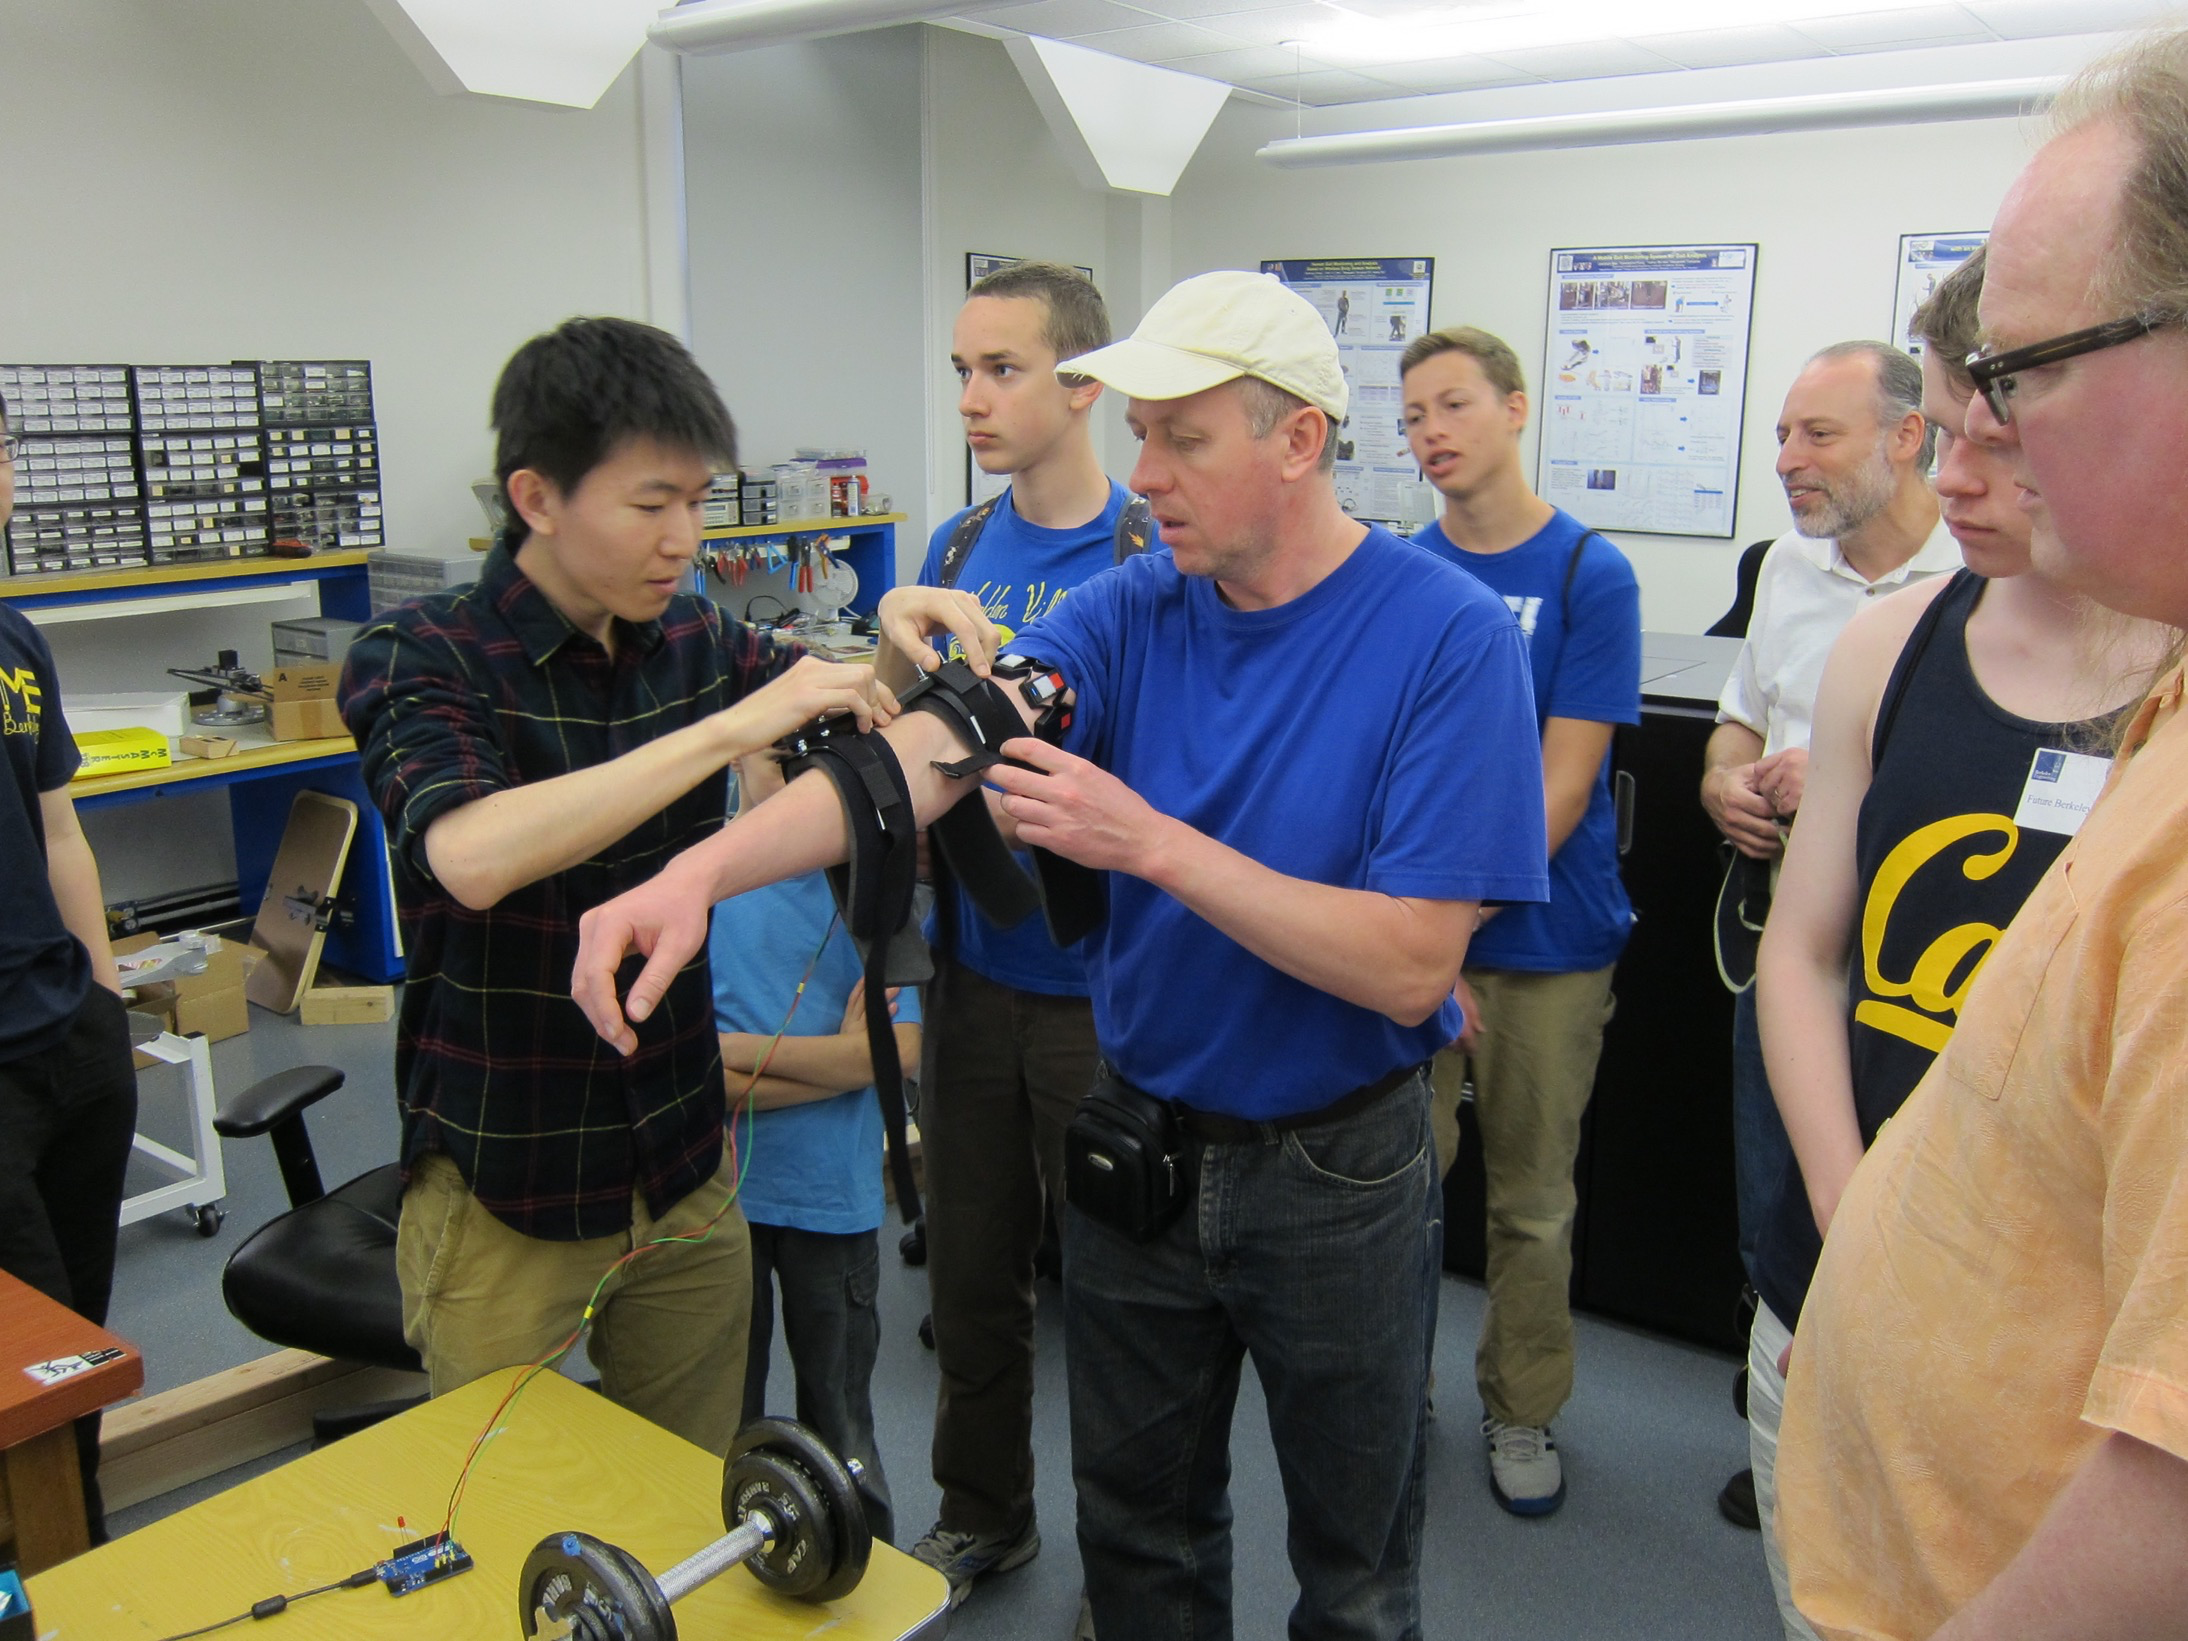
\includegraphics[width=4.5cm]{src/caldayphoto}
  \end{center}
  \vspace{-20pt}
  \caption{Cal Day 2016, a PhD student of Prof. Tomizuka demonstrating assistive technologies to visitors.\label{fig: cal day}}
  \vspace{-15pt}
\end{wrapfigure}

\paragraph*{Education Plan} ~
PI teaches robotics, design, and control courses both at the undergraduate and graduate levels emphasizing both theoretical principles and issues arising in applications of theory. His research students engage in laboratory work to acquire and develop experimental skills necessary to build, measure, and validate these new designs. 

\paragraph*{Involvement of Women and Minorities}~
The PI has a strong record in recruiting individuals from underrepresented groups, including women. While he was the Executive Associate Dean of the College of Engineering at UC Berkeley,  he was in charge of Engineering Student Services, one emphasis of which was (and still is) to broaden participation of the underrepresented groups. He has supervised twelve women to the completion of their Ph.D.s and currently supervises the Ph.D. research of nine women. 


\paragraph*{Outreach to Middle/High School Students}~
We will perform outreach to K-12 students and their parents though various official events of the University such as Cal Day (see Fig.\ref{fig: cal day} below). 
\paragraph*{Involvement of Undergraduate Students}~
Undergraduate students regularly participate in research work in the PI's lab, working closely with graduate students in projects involving hands-on experience in the fields of robotics and human mechatronics. The experimental test setups for the proposed project will provide an ideal example of interdisciplinary research, and will be made available to our undergraduate laboratory courses. The budget does not include a stipend for undergraduate researchers. We plan to request an REU supplement to attract undergraduate students from underrepresented backgrounds to the project.



\paragraph*{Broader Dissemination}~
We will disseminate the results from this research through the following mechanisms: 
(1) \textbf{Website}: Information about the group members, schedules of seminars, conferences, and workshops, copies of presentations, technical reports, code, and publications will be maintained at http://msc.berkeley.edu. The educational material, documentation, and the simulation platform developed will also be available through the website under an Open Source license. 
(2) \textbf{Journals and Conference Proceedings}: Research papers will be submitted for wide dissemination to journals and conferences in the field, such as the International Journal of Robotics Research, IEEE Transactions on Control System Technology, IEEE Intelligent Systems, IEEE Transactions of Robotics, IFAC Automatica, and ASME Journal of Dynamic Systems, Measurement, and Control.
(3) \textbf{Organized Laboratory Visits}: PI's MSC Lab regularly hosts various national and international student groups and visitors from universities and industry who will be presented with the results of the project.



\subsection{Results From Prior NSF Support}
% 5 pages or fewer of the 15 pages for entire description document.
% include results from NSF grants received in the past 5 years.
% If supported by more than one grant, choose the most relevant one.

% For each grant, include: 
%	(a) NSF award number, amount, dates of support 
%	(b) The title of this project
%	(c) Publications resulting from this research
%	(d) Summary of the results of the completed work
%	(e) A brief description of data samples available and other research products not described 	      elsewhere
%	(f) For renewed support, a description of the relationship between the completed and 			      proposed work

% Due to space limitations, it is often advisable to use citations rather
% than putting the titles of the publications in the body 
% of this section


%\paragraph*{\textit{IDR/Collaborative Research: Monitoring and Mobility Assistance with Wireless Body Sensor Network and Mechatronic Actuation}} (CMMI-1013657, September 1, 2010 - August 31, 2015, \$333,307)
%
%\textbf{Intellectual Merit}: This project studied a networked mobile assistive system (NMAS) by integrating a physical assistive device, a high-speed real-time wireless network, and a body sensor network. Major accomplishments were: 1) Prototype NMAS, 2) Control algorithms (e.g., modified LQG, model preview control, communication DOB) for a network-based rehabilitation system to deal with packet loss and varying time delay, 3) A tele-monitoring system (integration of smart shoes, IMUs, and XBee/RTWiFi/WirelessHART wireless network) for high-speed and real-time gait phase detection, and 4) Sensor fusion algorithms (e.g., time-varying complimentary filter, Direction-Cosine-Matrix estimation) using IMU sensors for accurate joint angle estimation. A preliminary clinical study conducted at the UC San Francisco demonstrated the effectiveness of NMAS in rehabilitation of patients with walking problems.
%
%\textbf{Broad Impact}: This proposed system will provide a comprehensive health care system to benefit both patients and health service providers by enabling mobile and tele-rehabilitation. Three graduate students (one of whom graduated with a Ph.D. degree), two postdoctoral researchers, and five undergraduate students have directly benefited from this project in PI Tomizuka's lab.  Four journal papers \cite{kong2012compact, bae2013tele, bae2013network, zhang2015modified} and many conference papers \cite{zhang2012modified, bae2012network, bae2012compensation, zhang2012design, zhang2013compensation, kanjanapas2013human, wei2013rt} have resulted from this project. We worked with multimedia group of the National Science Foundation to make a video of the wireless health monitoring system developed in this project \cite{nsf-video}.


\paragraph*{\textit{A Hybrid Control Systems Approach to Brain-Machine Interfaces for Exoskeleton Control}} (NSF-EFRI \#1137267, September 15, 2011 - August 31, 2015, \$2,000,000). 

\textbf{Intellectual Merit}: This interdisciplinary research addressed three major innovations (neurophysiology and brain-machine interfaces (BMI), hybrid control systems, and exoskeleton design and control) to significantly advance our understanding of fundamental principles in the neural control of movement in scenarios that involve physical interactions with the world. PI Tomizuka is mainly responsible for the third innovation (exoskeleton design and control). Major accomplishments in PI Tomizuka's lab include:
1) A passive 6-DOF upper-limb exoskeleton for macaques to test with the animals, 2) A cable-driven series elastic actuator and a torque-mode control algorithm for it, 3) An actuated version of the exoskeleton, and 4) An automatic 3D target positioner for BMI experiment use. The hybrid system approach is investigated for the BMI aspect (neural control and musculoskeletal model control).
 

\textbf{Broad Impact}: The three major innovations have been synthesized into a single new paradigm unifying the brain, biomechanics, and behavior. Two graduate students and four undergraduate students benefited from this project in PI Tomizuka's lab. The two graduate students completed their Ph.D. degrees.   Three journal papers \cite{lu2016design, lu2016interactive, haninger2016modelling} and several conference papers \cite{lu2013kinematic, haniger2014kinematic, lu2014passive, lu2014design, lu2015design, haninger2016motion, haninger2016robust} have resulted from this project. 

\paragraph*{\textit{Design of Mechanism and Control Strategies for Assistive Systems to Remedy the Decrease in Physical Strength of the Aged and the Disabled}} (CMMI \#1362172, August 1, 2014-July 31, 2017, \$307,074.00)

\textbf{Intellectual Merit}:  Integration of design and control of human assistive systems is emphasized in this research. The control problem is formulated from the viewpoint of a hybrid system. The research encompasses the segmentation of the dynamics of the human assistive system, the identification of transitions, and the development of control structures appropriate for each segment. To date, we have accomplished 1) development of a novel low-powered actuator for providing assistance; 2) Completion of a shoulder and elbow exoskeleton based on these low-power actuators; 3) Development of an algorithm for classifying the wearer's state whether the wearer has a load; and 4) Initial development of a controller for the device with the low-powered actuators by applying hybrid system theory.  Three conference papers have been published as a result of this project \cite{matthew2015introduction, matthew2015initial, matthew2015optimal}.

\textbf{Broad Impacts}: Existing work into assistive devices looks at either entirely passive assistance or fully active assistance. This new control framework uses individualized modeling to develop an active/passive actuator that can provide assistance without a large energy draw. Two Ph.D. students are working on this project and one of them graduated recently with his Ph.D. Four undergraduate students are participating.  % 
%%%%%%%%%%%%%% References no page limit %%%%%%%%%%%%%%%%%%%
\setcounter{page}{1}
\include{nsfref}
%%%%%%%%%%%%%% Postdoc Mentoring Plan%%%%%%%%%%%%%%%%%%%
%\setcounter{page}{1}
%\renewcommand{\thepage}{\arabic{page}}
\invisiblesection{Postdoc Mentoring Plan}
\begin{center}
\vspace{15pt}
\Large{\textbf{Postdoctoral Researcher Mentoring Plan}}
\end{center}

%Each proposal that requests funding to support postdoctoral researchers must include, as a supplementary document, a description of the mentoring activities that will be provided for
%such individuals. In no more than one page, the mentoring plan must describe the
%mentoring that will be provided to all postdoctoral researchers supported by
%the project, irrespective of whether they reside at the submitting organization,
%any subawardee organization, or at any organization participating in a
%simultaneously submitted collaborative project. Proposers are advised that the
%mentoring plan may not be used to circumvent the 15-page project description
%limitation.

\smallskip
%Examples of mentoring activities include, but are not limited to: career
%counseling; training in preparation of grant proposals, publications and presentations;
%guidance on ways to improve teaching and mentoring skills; guidance on how to
%effectively collaborate with researchers from diverse backgrounds and disciplinary areas;
%and training in responsible professional practices. The proposed mentoring activities
%will be evaluated as part of the merit review process under the broader impacts merit
%review criterion. Proposals that include funding to support postdoctoral researchers
%and do not include the requisite mentoring plan will be returned without review.


%Ms. Changliu Liu is currently at the final stage of her PhD study, and I plan to hire her as a post doctoral researcher for this project.  Ms. Liu is determined to develop an academic career, and she has a great potential to become an outstanding educator and researcher.  The primary emphasis during her PhD study was on her research.  Thus, I would like to provide her various opportunities to train her as an effective educator and researcher.  More specifically, my plans are as follows.
PI Tomizuka plans to hire a post doctoral researcher for this project. PI Tomizuka would like to provide the post doctoral researcher various opportunities to train him or her as an effective educator and researcher. More specifically, the plans are as follows.
\begin{enumerate}
\item PI Tomizuka will provide the post doctoral researcher opportunities to supervise graduate students and undergraduate student researchers on the topic of this NSF project. The project has become popular among students and PI Tomizuka is constantly approached by MS and undergraduate students volunteering their time and effort for experience. This does not mean that PI Tomizuka totally delegates to the post doctoral researcher his duty to supervise research students. The post doctoral researcher supervises these students on daily basis, and PI Tomizuka meets the post doctoral researcher and other students at regularly scheduled weekly research meetings and one-on-one individual meetings to provide his advice. 
\item In addition to students involved in this project, PI Tomizuka will let the post doctoral researcher develop interactions with students on other projects and to help their research. This will give the post doctoral researcher opportunities to improve skills for interacting with student, to learn other research projects and to develop a broad perspective on mechatronics research.  Other projects actively pursued in PI Tomizuka's research group include: autonomous driving, intelligent control of robot manipulators, building temperature control, and mechatronics for human assistance.
\item In April every year, University of California at Berkeley hosts CalDay, an open house of the Berkeley campus to general public including K-12 students.  PI Tomizuka's laboratory is a participant of this event every year. PI Tomizuka will ask the post doctoral researcher to play a leading role in this activity. By serving as the leader of PI Tomizuka's research group, the post doctoral researcher will be able to develop deep understanding of outreach activities.  
\end{enumerate}


%\bigskip
%\textbf{Documentation of collaborative arrangements} of significance to the
%proposal through letters of commitment.
%
%\smallskip
%%Proposers are reminded that, unless required by a specific program solicitation,
%%letters of support should not be submitted as they are not a standard component
%%of an NSF proposal, and, if included, a reviewer is under no obligation to review
%%these materials. Letters of support submitted in response to a program solicitation
%%requirement must be unique to the specific proposal submitted and cannot be altered
%%without the author's explicit prior approval. NSF may return without review proposals
%%that are not consistent with these instructions.
%
%\bigskip
%\textbf{Documentation regarding research involving the use of human subjects}, hazardous
%materials, vertebrate animals, or endangered species.

%%%%%%%%%%%%%% Biosketch  Max two pages per person%%%%%%%%%%%%%%%%%%%
%\setcounter{page}{1}
%%%%%%%%%%% Personnel
\renewcommand{\thepage}{\arabic{page}}
\section{List of Project Personnel}
\vspace{20pt}

\begin{enumerate}
\item PI: Masayoshi Tomizuka, University of California at Berkeley.
%\item Graduate student researcher: Changliu Liu, University of California at Berkeley.
%\item Graduate student researcher: TBN, University of California at Berkeley.
\end{enumerate}

%\invisiblesection{Facilities and Other Resources}

\setcounter{page}{1}
%\renewcommand{\thepage}{Facilities, Equipment, and Other Resources - Page \arabic{page} of 1}

\begin{center}
\textbf{\large Facilities, Equipment \& Other Resources}
\end{center}

%	Identify the facilities to be used, as appropriate, indicate their capacities,
%	pertinent capabilities, relative proximity, and extent of availability to the project.
%	Use ``Other" to describe the facilities at any other performance sites listed and at
%	sites for field studies.

% \textbf{Laboratory:}
% 
% \textbf{Clinical:}
% 
% \textbf{Animal:}

PI Tomizuka's Mechanical Systems Control (MSC) Laboratory includes facilities to support theoretical analysis and software development for the safe and efficient robot collaboration system (SERoCS). In particular, the laboratory has the following capabilities:

\begin{enumerate}
\item Computers: Networked PCs running Windows XP/Windows 7/Ubuntu, deep learning workstation with four NVIDIA Titan X Pascal;
\item Control \& data acquisition facilities: National Instrument LabVIEW FPGA Pioneer System, National Instrument LabVIEW RealTime Module, National Instrument compact RIO, Single-Board RIO, National Instrument data acquisition boards, and Simulink Real-Time target computer;
\item Sensors: one PhaseSpace Impulse X2 Motion Capture system, two Microsoft Kinect stereo cameras and two IDS Ensenso N35 stereo cameras;
\item Robots: Two FANUC LR Mate 200\textit{i}D/7L robots with SMC LEHF grippers and ATI mini 45 force / torque sensors, and one FANUC M-16\textit{i}B robot arm.\end{enumerate}
The MSC laboratory has a floor space of about $3,200 ft^2$, which is adequate for performing all planned experiments using mobile robots.
The PIs also have access to 3D printing and Fused Deposition Modeling (FDM) machines for rapid- prototyping through the ME Department and the Center for Information Technology Research in the Interest of Society (CITRIS) at UC Berkeley. The 3D printer in the ME department can manufacture objects up to 10" x 10" x 12" while the 3D printer at CITRIS can print objects in the size of 8" x 8" x 12".

%% Supplementary Documents
%%%%%%%%%%%%% Data Management 1 page REQUIRED
%\setcounter{page}{1}
%\setcounter{page}{1}
\renewcommand{\thepage}{\arabic{page}}
%\required{Supplementary Documentation}
\invisiblesection{Data Management Plan}

~
\vspace{-15pt}
\begin{center}
\Large{\textbf{Data Management Plan}}
\end{center}
% Maximum of 2 pages
%------------------------------

% This supplement should describe how the proposal will conform to NSF policy on
% the dissemination and sharing of research results and may include:
% 
% 1. The types of data, samples, physical collections, software, curriculum
%    materials, and other materials to be produced in the course of the project;
% 
% 2. The standards to be used for data and metadata format and content (where
%    existing standards are absent or deemed inadequate, this should be documented
%    along with any proposed solutions or remedies);
% 
% 3. Policies for access and sharing including provisions for appropriate
% protection   of privacy, confidentiality, security, intellectual property, or
% other rights or   requirements;
% 
% 4. Policies and provisions for re-use, re-distribution, and the production of
%    derivatives; and
% 
% 5. Plans for archiving data, samples, and other research products, and for
%    preservation of access to them.
% 
% A valid Data Management Plan may include only the statement that no detailed
% plan is needed, as long as the statement is accompanied by a clear
% justification. Proposers who feel that the plan cannot fit within the supplement
% limit of two pages may use part of the 15-page Project Description for
% additional data management information. Proposers are advised that the Data
% Management Plan may not be used to circumvent the 15-page Project Description
% limitation.

\subsection{Types of Data}
In this project, the following types of data are expected to be generated:

\subsubsection*{(1) Data to Be Collected and the Cognition Model Library in T1.1}
\begin{itemize} \itemsep0pt \parskip0pt \parsep0pt
\item Trajectory of human motion in different scenarios and tasks;
\item Identified human behavior types and the associated features;
\item Identified human behavioral models;
\end{itemize}
\vspace{-10pt}


\subsubsection*{(2) Data to Be Collected and the Motion Skill Library in T2.1}
\begin{itemize} \itemsep0pt \parskip0pt \parsep0pt
\item Force and motion trajectory of human demonstrations in different scenarios and tasks;
\item Identified motion skill models and the associated features;
\end{itemize}
\vspace{-10pt}

\subsubsection*{(3) Algorithms in Processing the Data in T1.1 and T2.1}
\begin{itemize} \itemsep0pt \parskip0pt \parsep0pt
\item C++/Matlab/Python source code of the classification algorithm of human behavior and the model extraction algorithm;
\item C++/Matlab/Python source code of the supervised learning algorithm of skill model training;
\end{itemize}
\vspace{-10pt}

\subsubsection*{(4) Algorithms to Be Developed in T1.2, T2.2 and T3.1}

\begin{itemize} \itemsep0pt \parskip0pt \parsep0pt
\item C++/Matlab/Python source code of the online learning algorithm of stochastic time-varying systems;
\item C++/Matlab/Python source code of the online task planning algorithm;
\item C++/Matlab/Python source code of the efficiency controller;
\item C++/Matlab/Python source code of the safety controller;
\end{itemize}

\vspace{-10pt}

\subsubsection*{(5) The Evaluation Platforms to Be Developed in T4.1}

\begin{itemize} \itemsep0pt \parskip0pt \parsep0pt
\item Source code of Platform 1 to Platform 5;
\item The executable software;
\item User manual;
\end{itemize}

\vspace{-10pt}


\subsubsection*{(6) Documents and Others}

\begin{itemize} \itemsep0pt \parskip0pt \parsep0pt
\item Questionnaires;
\item Curriculum materials from courses taught, and talks given at seminars / tutorials / etc.
\item Publications intended for public dissemination;
\end{itemize}

\subsection{Standards}
Standard commercially available hardware (e.g., cameras, computers, displays, sensors) will be used in the study, as well as standard commercially available operating systems, such as Windows, MAC OS and Linux distributions. The source code will be written in Matlab, C/C++, and Python with support from some of the Open Source libraries (e.g. OpenCV). For communication purposes we will use TCP/IP.

Data will be stored in standard formats provided by the equipment manufacturers. (1) The algorithm related data will be stored in ASCII text format. (2) The images will be stored in standard formats, such as PGM and PPM in standard resolutions (VGA or QVGA). (3) Motion trajectories will be stored in ASCII text format or custom documented binary formats for efficiency. (4) For the data compression, ZIP compression algorithms will be used. (5) The documentation for the framework will be stored in DOC, TEX format and distributed in standard PDF format.


\subsection{Policies for Access}
All study protocols will be approved by the University Institutional Review Board (IRB) prior to performance, and all research guidelines and rules will be strictly adhered to for both privacy and protection of human subjects and data for research.

The access to the data will be secured via SSH protocols and individual access will be given to the participating researchers. The server for the source code will not hold any human subject information. Any information on subjects will be anonymized and stored on computers with password protection. Any information on subjects that could be linked to individuals will be encrypted (e.g. using AES-256 algorithm). The human behavioral data (anonymized) will be provided to other researchers for academic use to evaluate their learning and control algorithms. Registrations will be required.


\subsection{Policies for Re-use and Re-distribution}
The source code data will be handled by academic licenses and provided free for non-profit (academic) software use, reserving rights of UC Berkeley for commercial use. Users will be required to register. The software copyright notice will be as follows: http://ipira.berkeley.edu/software-copyright-notice-and-disclaimer. Data and programs will be shared in a timely manner (typically within a few months of the relevant paper being published). Curriculum materials will be made available in a timely manner at the PI's web pages or course web pages, as permitted by UC Berkeley, with no restrictions for re-use (provided that authors are acknowledged).


\subsection{Plans for Dissemination and Archiving the Data}
For archiving and storage of source code and data, we have a dedicated experimental PC which is regularly backed up to an external device/storage.
The dissemination of the stable version of software will proceed after the publication and protection of IP from each partner and publication. The human behavioral data will also be shared with the academic community after the publications upon the permission of the subject.
We believe it is important to maintain data access along the life of the project. We will provide data distributions based on a long-term web host supported by UC Berkeley. We will use campus-provided services for backups of the data.
%%%%%%%%%%REU Description if requesting REU - 3 page max
%\setcounter{page}{1}
%\setcounter{page}{1}
\renewcommand{\thepage}{\arabic{page}}
\invisiblesection{Human Subjects Protection Plan}

~
\vspace{-15pt}
\begin{center}
\Large{\textbf{Human Subjects Protection Plan}}
\end{center}
\subsection{Risks to Subjects}

We will include human subject participation in three ways: (1) construction of the cognition model library in T1, (2) construction of the motion skill library in T2, (3) evaluation of the SERoCS on Platforms 1-3 in T4, and (4) evaluation of the SERoCS on Platform 5 in T4.

\textbf{Construction of the cognition model library in T1}. The experiment in collecting human motion data will be performed inside PI Tomizuka's Mechanical Systems Control Lab at UC Berkeley. The subject's motion will be captured by vision cameras. There is no risk to the subject during the study.

\textbf{Construction of the motion skill library in T2}. The human demonstration will be performed inside PI Tomizuka's Mechanical Systems Control Lab at UC Berkeley. The subject will be asked to (1) wear motion capture suits or gloves, and perform remote demonstrations of multiple types of tasks, (2) grasp the robot end-effector, and perform direct demonstrations by lead through teaching. There is a potential risk of physical injury from collision between the robot and the subject. Several safeguarding mechanisms, as will be described below, will be in place to reduce such risks.

\textbf{Evaluation of the SERoCS on Platforms 1-3 in T4}. The evaluation and testing will be performed inside PI Tomizuka's Mechanical Systems Control Lab at UC Berkeley. The subject interacts with the robot virtually. There is no risk to the subject during the study.

\textbf{Evaluation of the SERoCS on Platform 5 in T4}. The evaluation and testing will be performed inside PI Tomizuka's Mechanical Systems Control Lab at UC Berkeley. The subject will be asked to perform (1) simple tasks (sitting on a chair, walking around) inside the robot's workspace and (2) joint tasks (lift/move/rotate one workpiece) with the robot. There is a potential risk of physical injury from collision between the robot and the subject. Several safeguarding mechanisms, as will be described below, will be in place to reduce such risks.

\textbf{Confidentiality}. There is a potential risk of loss of confidentiality from participation in these experiments.

\subsection{Plans for Recruitment and Informed Consent}
Subjects will be evaluated in PI Tomizuka's Mechanical Systems Control Lab at UC Berkeley. 5-10 healthy adult volunteers (ages 18-60) will be recruited for the experiment, including 3-5 experienced workers who are familiar with robotics.

All subjects will undergo informed consent procedures based on the approval of the University Institutional Review Board (IRB). Consent documents will present a complete review of study background, aims, procedures, potential risks and benefits, study costs, rights of research participants, and study staff contact information. The experiments will be conducted in accordance with regulatory requirements regarding involvement of human subjects in research. All subject testing protocols, consent documents, and patient materials will be reviewed and approved by the UC Berkeley Committee for Protection of Human Subjects.

\subsection{Inclusion of Women, Minorities, and Children}
The inclusion of women, minorities, and children will be considered as follows:

\textbf{Inclusion of Women}. Both men and women will be recruited for this study, whereas equal number of
men and women will be included, for an adequate sample size of men and women to address gender differences with respect to evaluation procedures and task performance.

\textbf{Inclusion of Minorities}. The study does not exclude volunteers on the basis of race or ethnicity. The demographic mix or racial and ethnic groups is well represented at UC Berkeley as well as in the local communities. Attempts will be made to recruit subjects with a similar ethnic and racial diversity to that of the general population in the respective areas.

\textbf{Inclusion of Children}. Since the project is aimed at evaluating robots' safety performances in a factory environment, we do not plan to include individuals of less than 18 years of age.


\subsection{Planned Procedures to Protect Against and Minimize Potential Risks}
To protect against and to minimize potential risks to human subjects, the following mechanisms will be in place:

\textbf{Construction of the motion skill library}.
(1) Emergency check (including threshold monitoring of joint position, velocity and torque, collision prediction and detection)  and various software failure protocols will be developed and implemented under different task scenarios. The robot should stop immediately if emergency or software failure is detected.  (2) Prior to the experiments with the robot, the human subjects will be trained (i) using the simulation platforms, e.g. Platform 1 and Platform 2, and (ii) by indirect interaction with the robot arm in Platform 3, i.e. requiring the subjects to control a mobile robot to interact with the robot arm. (3) Subjects will be required to wear helmets and goggles during the experiments. (4) A research staff will monitor the experiment and will stop the robot in emergencies. (6) Questionnaires will be sent out after the tests to address potential issues related to subject's comfort and acceptance of the collaborative robot and the SERoCS.

\textbf{Evaluation of the SERoCS on Platform 5 with the mobile robot}. (1) The experiment will be performed only if the SERoCS demonstrates success in the Platforms 1-3. (2) Prior to the experiments with the mobile robot, the human subjects will be trained (i) using the simulation platforms, e.g. Platform 1 and Platform 2 and (ii) by indirect interaction with the testing mobile robot in Platform 3, i.e. requiring the subjects to control another mobile robot to interact with the testing mobile robot. (3) Subjects will be required to wear helmets and goggles during the experiments. (4) Emergency checks and various software failure protocols will be implemented under different task scenarios. (5) A research staff will monitor the experiment and will take charge of the control of the testing mobile robot in emergencies. (6) Questionnaires will be sent out after the tests to address potential issues related to subject's comfort and acceptance of the SERoCS.

\textbf{Evaluation of the SERoCS on Platform 5 with the robot arm}. 
(1) The experiment will be performed only if the SERoCS demonstrates success in the simulation platforms. (2) Prior to the experiments with the robot arm, the human subjects will be trained (i) using the simulation platforms, e.g. Platform 1 and Platform 2, and (ii) by indirect interaction with the robot arm in Platform 3, i.e. requiring the subjects to control a mobile robot to interact with the robot arm. (3) Subjects will be required to wear helmets and goggles during the experiments. (4) A research staff will monitor the experiment and will stop the robot in emergencies.
(5) Emergency check and various software failure protocols will also be implemented under different task scenarios. (6) Questionnaires will be sent out after the tests to address potential issues related to subject's comfort and acceptance of the collaborative robot and the SERoCS.

\textbf{Confidentiality}. No personal identifiable information will be collected on the subjects. In addition to the sensor data we will collect anthropometric data (e.g., height), demographic data (e.g., age, sex) and data indicating whether the subject is experienced in the field of robotics or not. All the data will be anonymized in the process. The data will be stored on secured servers. Only the PI Prof. Tomizuka, and the researcher(s) working on this project will have access to the personal data. This information will be stored in locked cabinets and/or password protected computers in their respective offices. For the public dissemination of the sensor data, we will minimize potential risks of loss of confidentiality by coding all subjects and their recordings.





%
%\bibliography{nsf-nri}
\end{document}